\documentclass{article}
\usepackage[paperheight=30cm,textheight=25cm]{geometry}
\usepackage[dvipsnames]{xcolor}
\usepackage{amsmath,graphicx}
\usepackage{tikzinput,wrapfig,mdframed,listings}
\usepackage[most]{tcolorbox}
\usepackage{mdframed}

% ------------------------------------------------------------------

\def\red{\textcolor{red}}
\def\blue{\textcolor{blue}}
\def\gray{\textcolor{gray}}
\def\green{\textcolor{ForestGreen}}
\def\orange{\textcolor{YellowOrange}}
\def\purple{\textcolor{RedViolet}}

\def\loremI{Lorem ipsum dolor sit amet, consectetur adipiscing elit. 
Pellentesque sed diam ex. Nam pretium sagittis lacus, et consequat lacus 
interdum in. In molestie porttitor purus, ac euismod quam cursus id. 
Sed facilisis eget enim in varius.}
%In faucibus mauris libero, ut 
%interdum dolor tristique nec. Vivamus pellentesque laoreet risus, 
%quis volutpat enim congue tincidunt. Praesent vel mi sed lectus pharetra 
%vestibulum a eu quam. Nunc elementum ac eros nec tempor. Nullam faucibus 
%neque non eros tristique, vitae malesuada urna euismod. In hac habitasse 
%platea dictumst. Integer aliquam condimentum tellus, non tincidunt enim 
%iaculis non. Nunc ullamcorper eleifend nunc, ac ultricies eros lobortis 
%finibus. Quisque ipsum erat, viverra at ligula eu, placerat varius eros.
%Aliquam dapibus dapibus dolor, nec fringilla lectus lobortis vitae. 
%Nulla nec tincidunt quam, vitae luctus ipsum. Phasellus rutrum turpis 
%non dui maximus vestibulum. Vivamus quis ultrices libero, vitae 
%rhoncus ex. Duis fringilla elit et euismod congue. Suspendisse blandit 
%nibh ac ante auctor vehicula. Nam sit amet auctor nisi, et malesuada 
%turpis. Praesent pellentesque hendrerit leo nec rutrum. Suspendisse eu 
%sem sem.}
\def\lorem{\gray\loremI}

\long\def\showpar#1{\lorem{} #1 {}\lorem\medskip\par}

\long\def\showhinner#1{\blue{\textbackslash hbox\{}#1\blue{\}}}
\long\def\showh#1{\hbox{\showhinner{#1}}}
\long\def\showhto#1#2{\hbox to#1{\showhinner{#2}}}
\long\def\showhwith#1#2#3#4{\boxwith{#1}{#2}{#3}{\showh{#4}}}

\long\def\showvinner#1{\hbox{\red{\textbackslash vbox\{}}#1\hbox{\red{\}}}}
\long\def\showv#1{\vbox{\showvinner{#1}}}
\long\def\showvto#1#2{\vbox to#1{\showvinner{#2}}}
\long\def\showvwith#1#2#3#4{\boxwith{#1}{#2}{#3}{\showv{#4}}}

\long\def\showtinner#1{\hbox{\red{\textbackslash vtop\{}}#1\hbox{\red{\}}}}
\long\def\showt#1{\vtop{\showtinner{#1}}}
\long\def\showtto#1#2{\vtop to#1{\showtinner{#2}}}
\long\def\showtwith#1#2#3#4{\boxwith{#1}{#2}{#3}{\showt{#4}}}

\long\def\showcinner#1{\hbox{\red{\textbackslash vcenter\{}}#1\hbox{\red{\}}}}
\long\def\showc#1{\vcenter{\showcinner{#1}}}
\long\def\showcto#1#2{\vcenter to#1{\showcinner{#2}}}
\long\def\showcwith#1#2#3#4{\boxwith{#1}{#2}{#3}{\showc{#4}}}

\long\def\block#1#2{\par\noindent\textbf{#1}\smallskip\par\hrule width\textwidth
  \relax#2\par\hrule width\textwidth\bigskip
}
\def\conclude#1{%
  \green{\begin{itemize}\item[$\Rightarrow$]#1\end{itemize}\medskip}%
}
\def\cs#1{\orange{\texttt{\textbackslash#1}}}
\def\meta#1{\purple{$\langle$\texttt{#1}$\rangle$}}

\ExplSyntaxOn
\long\def\boxwith#1#2#3#4{
  \setbox0#4
  \tl_if_empty:nF{#1}{\wd0=#1}
  \tl_if_empty:nF{#2}{\ht0=#2}
  \tl_if_empty:nF{#3}{\dp0=#3}
  \box0
}
\ExplSyntaxOff

\parindent=15pt

\newbox\mynumbox

\def\mynum#1{\setbox\mynumbox\hbox{\hskip-20pt #1.}\wd\mynumbox=0pt\ht\mynumbox=0pt\dp\mynumbox=0pt\box\mynumbox}

\usepackage{ded}

% ------------------------------------------------------------------

\begin{document}
\ifx\rustexBREAK\undefined
  \let\rustexBREAK\relax
\fi

\section{ridiculousness}
\hrule
\vbox to 50px {
	\hbox{foo}
	\vskip 50px minus -50pt
	\hbox{bar}
}
\hrule

\section{Arithmetics}

\begingroup


\newcount\tint
\newdimen\tdim
\newcount\tempint
\newdimen\tempdim


\def\line{%
  \global\advance\tint1
  \global\advance\tdim1sp
  \the\tint & \the\tdim &
  	\tempint=\tint\relax
  	\divide\tint by 2
  	\the\tint &
  	\tempint=\tint\relax
  	\multiply\tint by 2
  	\divide\tint by 3
  	\the\tint &
  	\tempdim=\tdim\relax
  	\divide\tdim by 2
  	\the\tdim &
  	\tempdim=\tdim\relax
  	\multiply\tdim by 2
  	\divide\tdim by 3
  	\the\tdim &
  	\tempdim=0.5\tdim\relax
  	\the\tempdim &
  	\the\numexpr\tint/2\relax &
  	\the\numexpr\tint*2/3\relax &
  	\the\dimexpr\tdim/2\relax &
  	\the\dimexpr\tdim*2/3\relax \cr%
}

\halign{\hskip-50pt#\hskip10pt & #\hskip10pt & #\hskip10pt & #\hskip10pt & #\hskip10pt & #\hskip10pt & #\hskip10pt & #\hskip10pt & #\hskip10pt & #\hskip10pt & #\hskip10pt \cr
\textbf{count} & \textbf{as pt} & \textbf{c/2} & \textbf{c*2/3} & \textbf{d/2} & \textbf{d*2/3} & \textbf{0.5d} &
\textbf{e c/2} & \textbf{e c*2/3} & \textbf{e d/2} & \textbf{e d*2/3} \cr
	\line\line\line\line\line\line\line\line\line\line\line\line
	\line\line\line\line\line\line\line\line\line\line\line\line
	\line\line\line\line\line\line\line\line\line\line\line\line
}

\tempdim=1.0sp
\noindent sp: \the\numexpr\tempdim\relax\par
\tempdim=1.0pt
\noindent pt: \the\numexpr\tempdim\relax\par
\tempdim=1.0pc
\noindent pc: \the\numexpr\tempdim\relax\par
\tempdim=1.0in
\noindent in: \the\numexpr\tempdim\relax\par
\tempdim=1.0bp
\noindent bp: \the\numexpr\tempdim\relax\par
\tempdim=1.0cm
\noindent cm: \the\numexpr\tempdim\relax\par
\tempdim=1.0mm
\noindent mm: \the\numexpr\tempdim\relax\par
\tempdim=1.0dd
\noindent dd: \the\numexpr\tempdim\relax\par
\tempdim=1.0cc
\noindent cc: \the\numexpr\tempdim\relax\par

\pagebreak

\begingroup\makeatletter
\newdimen\pgf@x
\newdimen\pgf@y
\newdimen\pgf@xa
\newdimen\pgf@ya
\newdimen\pgf@xb
\newdimen\pgf@yb
\newdimen\pgf@xc
\newdimen\pgf@yc

\pgf@x=14.3879pt
\pgf@y=2.02766pt
\def\pgf@time@s{0.47308}
\def\pgf@time@t{0.52692}

\pgf@xa=36.11493pt
\pgf@ya=5.09137pt
\pgf@xb=49.23415pt
\pgf@yb=5.09137pt
\pgf@xc=70.96172pt
\pgf@yc=2.02765pt

\def\line{\the\pgf@x & \the\pgf@y & \the\pgf@xa & \the\pgf@ya & \the\pgf@xb & \the\pgf@yb & \the\pgf@xc & \the\pgf@yc \cr }

\halign{ #\hskip10pt & #\hskip10pt & #\hskip10pt & #\hskip10pt & #\hskip10pt & #\hskip10pt & #\hskip10pt & #\hskip10pt \cr 
\textbf{pgf@x} & \textbf{pgf@y} & \textbf{pgf@xa} & \textbf{pgf@ya} & \textbf{pgf@xb} & \textbf{pgf@yb} & \textbf{pgf@xc} & \textbf{pgf@yc} \cr
\line
\global\pgf@x =\pgf@time@t\pgf@x
\line
\global\advance \pgf@x by\pgf@time@s \pgf@xa 
\line
\global\pgf@y =\pgf@time@t \pgf@y 
\line
\global\advance \pgf@y by\pgf@time@s \pgf@ya 
\line
\global\pgf@xa =\pgf@time@t \pgf@xa 
\line
\global\advance \pgf@xa by\pgf@time@s \pgf@xb 
\line
\global\pgf@ya =\pgf@time@t \pgf@ya 
\line
\global\advance \pgf@ya by\pgf@time@s \pgf@yb 
\line
\global\pgf@xb =\pgf@time@t \pgf@xb 
\line
\global\advance \pgf@xb by\pgf@time@s \pgf@xc 
\line
\global\pgf@yb =\pgf@time@t \pgf@yb 
\line
\global\advance \pgf@yb by\pgf@time@s \pgf@yc 
\line
\global\pgf@x =\pgf@time@t \pgf@x 
\line
\global\advance \pgf@x by\pgf@time@s \pgf@xa 
\line
\global\pgf@y =\pgf@time@t \pgf@y 
\line
\global\advance \pgf@y by\pgf@time@s \pgf@ya 
\line
\global\pgf@xa =\pgf@time@t \pgf@xa 
\line
\global\advance \pgf@xa by\pgf@time@s \pgf@xb 
\line
\global\pgf@ya =\pgf@time@t \pgf@ya 
\line
\global\advance \pgf@ya by\pgf@time@s \pgf@yb 
\line
\global\pgf@xb =\pgf@x 
\line
\global\pgf@yb =\pgf@y 
\line
\global\pgf@x =\pgf@time@t \pgf@x 
\line
\global\advance \pgf@x by\pgf@time@s \pgf@xa 
\line
\global\pgf@y =\pgf@time@t \pgf@y 
\line
\global\advance \pgf@y by\pgf@time@s \pgf@ya 
\line
}

\endgroup
\endgroup
\pagebreak

%% ---------------------------------------------------------------

\section{Boxes}

\subsection{HBoxes}

\block{HBox:}{%
  \showhwith\textwidth{}{}{ Box Content }

  \setbox0\hbox to 150pt{\showhinner{ Box Content }}
  \wd0=\textwidth\box0

  \showhto\textwidth{ Box Content }

  \showhto\textwidth{ \showhwith\textwidth{}{}{ Box Content } }

  \setbox0\hbox to 150pt{ \showhinner{ Box Content } }
  \wd0=\textwidth\showhto\textwidth{ \box0 }
  
  \showhto\textwidth{ \showhto\textwidth{ Box Content } }

  \hbox to\textwidth{ BoxContent}

  \showhto\textwidth{%
    \showhwith{20pt}{}{}{ Box Content }................................\hskip50pt%
    \showhto{20pt}{ Box Content }................................\hskip50pt%
  }
  \showhwith{}{40pt}{}{ Box Content }

  \hbox spread 0.5\textwidth{\showhinner{ Box Content }}
  \showh{\showhwith{-20pt}{}{}{Box Content}}
  \showh{\showhto{-20pt}{Box Content}}
}

\block{In Paragraphs:}{
\noindent \showpar{\hbox to100pt{Some Box Content}}

\noindent \showpar{\setbox0\hbox to150pt{Some Box Content}\unhbox0}

\noindent \showpar{\hbox spread50pt{Some Box Content}}

\noindent \showpar{\setbox0\hbox to50pt{ Box }\wd0=100pt\ht0=50pt\dp0=25pt\box0}

\noindent \showpar{\setbox0\hbox to50pt{ \showv{%
\hbox{Content}\hbox{Content}\hbox{Content}\hbox{Content}%
  } }\wd0=100pt\ht0=50pt\dp0=25pt\box0}
}

%% ---------------------------------------------------------------
\pagebreak


\subsection{VBoxes}

\block{}{
  \showh{\showv{\hbox{Content}}}
  \noindent\showpar{\showv{\hbox{Content}}}
  \noindent\showpar{\showh{\showv{\hbox{Content}}}}
}

\block{Height}{
  \showh{\showvwith{}{50pt}{}{\hbox{Content}}}
  \noindent\showpar{\showvwith{}{50pt}{}{\hbox{Content}}}
  \noindent\showpar{\showh{\showvwith{}{50pt}{}{\hbox{Content}}}}
}
\pagebreak

\block{Depth}{
  \showh{\showvwith{}{}{30pt}{\hbox{Content}}}
  \noindent\showpar{\showvwith{}{}{30pt}{\hbox{Content}}}
  \noindent\showpar{\showh{\showvwith{}{}{30pt}{\hbox{Content}}}}
}

\block{Height and Depth:}{
  \showh{\showvwith{}{50pt}{30pt}{\hbox{Content}}}
  \noindent\showpar{\showvwith{}{50pt}{30pt}{\hbox{Content}}}
  \noindent\showpar{\showh{\showvwith{}{50pt}{30pt}{\hbox{Content}}}}
}
\pagebreak

\block{To and Depth:}{
  \showh{\setbox0\vbox to 50pt{\showvinner{\hbox{Content}}}%
    \dp0=30pt\box0}
  \noindent\showpar{\setbox0\vbox to 50pt{\showvinner{\hbox{Content}}}%
    \dp0=30pt\box0}
  \noindent\showpar{\showh{\setbox0\vbox to 50pt{\showvinner{\hbox{Content}}}%
    \dp0=30pt\box0}}
}

\block{Height with Para:}{
  \showh{\showvwith{}{80pt}{}{\noindent\lorem\par}}
}
\block{To with Para:}{
  \showh{\showvto{80pt}{\noindent\lorem\par}}
}
\block{Small Height with Para:}{
  \showh{\showvwith{}{5pt}{}{\noindent\lorem\par}}
}
\vskip40pt
\noindent(\cs{vskip})
\pagebreak

\block{Small Height with Depth and Para:}{
  \showh{\showvwith{}{5pt}{40pt}{\noindent\lorem\par}}
}

\block{VBox with To and Height and Depth:}{
  \showh{\setbox0\vbox to 50pt{\showvinner{\noindent\lorem\par}}%
    \dp0=30pt\box0}
}

\block{Para in \cs{vbox} in Para}{\showpar{\showvwith{50pt}{}{}{\showpar{}}}}

\block{VBoxes:}{\showh{%
  \showvwith{}{150pt}{}{\hbox{Box Content}}%
  \showvto{150pt}{\hbox{Box Content}}
  \setbox0\vbox to100pt{\showvinner{ \hbox{ Box Content } }}%
  \ht0=150pt\box0%
  \setbox0\vbox to100pt{\showvinner{ \hbox{ Box Content } \noindent\lorem\par }}%
  \ht0=150pt\box0%
}}


%\conclude{\meta{to} $\neq$ \meta{height}; top-aligned, but %paragraphs 
%have \cs{vfil} above.}
\pagebreak

\subsection{VTops}

\block{}{
  \showh{\showt{\hbox{Content}}}
  \noindent\showpar{\showt{\hbox{Content}}}
  \noindent\showpar{\showh{\showt{\hbox{Content}}}}
}

\block{Height}{
  \showh{\showtwith{}{50pt}{}{\hbox{Content}}}
  \noindent\showpar{\showtwith{}{50pt}{}{\hbox{Content}}}
  \noindent\showpar{\showh{\showtwith{}{50pt}{}{\hbox{Content}}}}
}
\pagebreak

\block{Depth}{
  \showh{\showtwith{}{}{10pt}{\hbox{Content}}}
  \showh{\showtwith{}{}{50pt}{\hbox{Content}}}
  \noindent\showpar{\showtwith{}{}{50pt}{\hbox{Content}}}
  \noindent\showpar{\showh{\showtwith{}{}{10pt}{\hbox{Content}}}}
}

\block{Height and Depth:}{
  \showh{\showtwith{}{50pt}{10pt}{\hbox{Content}}}
  \noindent\showpar{\showtwith{}{50pt}{50pt}{\hbox{Content}}}
  \noindent\showpar{\showh{\showtwith{}{50pt}{10pt}{\hbox{Content}}}}
}
\pagebreak

\block{To and Depth:}{
  \showh{\setbox0\vtop to 50pt{\showtinner{\hbox{Content}}}%
    \dp0=10pt\box0}
  \noindent\showpar{\setbox0\vtop to 50pt{\showtinner{\hbox{Content}}}%
    \dp0=50pt\box0}
  \noindent\showpar{\showh{\setbox0\vtop to 50pt{\showtinner{\hbox{Content}}}%
    \dp0=10pt\box0}}
}

\block{Height with Para:}{
  \showh{\showtwith{}{80pt}{}{\noindent\lorem\par}}
}
\block{To with Para:}{
  \showh{\showtto{80pt}{\noindent\lorem\par}}
}
\block{Small Height with Para:}{
  \showh{\showtwith{}{10pt}{}{\noindent\lorem\par}}
}

\block{Small Height with Depth and Para:}{
  \showh{\showtwith{}{10pt}{40pt}{\noindent\lorem\par}}
}

\vskip20pt
\noindent(\cs{vskip})
\pagebreak

\block{VTop with To and Height and Depth:}{
  \showh{\setbox0\vtop to 50pt{\showtinner{\noindent\lorem\par}}%
    \dp0=30pt\box0}
}

\vskip20pt
\noindent(\cs{vskip})

\block{Para in \cs{vtop} in Para}{\showpar{\showtwith{50pt}{}{}{\showpar{}}}}



\block{VTops:}{\showh{%
  \showtwith{}{150pt}{}{\hbox{Box Content}}%
  \showtto{150pt}{\hbox{Box Content}}
  \setbox0\vtop to100pt{\showtinner{ \hbox{ Box Content } }}%
  \ht0=150pt\box0%
  \setbox0\vtop to100pt{\showtinner{ \hbox{ Box Content } \noindent\lorem\par }}%
  \ht0=150pt\box0%
}}


\pagebreak

\block{\cs{vtop} with Depth/Height in H}{%
  \showh{%
    \showtwith{}{50pt}{}{\hbox{Box Content}}%
    \showtwith{}{}{50pt}{\hbox{Box Content}}%
    \showtwith{}{50pt}{50pt}{\hbox{Box Content}}%
  }
}


\section{\cs{[v|h]rule}}

\block{\cs{hrule} in \cs{vbox} in \cs{hbox}}{
  \showh{ \showv{ \hrule width 50pt height 75pt depth 25 pt } }
}

\block{\cs{hrule} in \cs{vbox} with height in \cs{hbox}}{
  \showh{ \setbox0\showv{ \hrule width 50pt height 75pt depth 25 pt } \ht0=150pt\box0 }
}

\block{\cs{vrule} in \cs{hbox}}{
  \showh{ \vrule width 50pt height 75pt depth 25pt }
  \showh{ foo \vrule foo}
  \showh{\vrule \showv{\showh{}}\vrule}
  \hbox{\vrule}
  \vskip10pt
}
\pagebreak

\block{\cs{vrule} in Para without parameters}{
  \vskip10pt \noindent Here \vrule bla\par
  \noindent \vrule \par
  \noindent Here\par\vskip10pt
}

\block{\cs{vrule} in Para}{
  \showpar{ \vrule width 50pt height 75pt depth 25pt }
  \showpar{ \vrule width 10pt height 0.1pt \gray{lorem bla}
   \vrule width 10pt }
}

\block{\cs{hrule} in \cs{vbox}}{
  \showv{ \hrule }
}

\section{Math}

\def\mymath{\alpha + \mathop{\red\int}_{t=1}^\infty \mathop{\blue\sum}_{x=0}^N f(t,x)^t_x
  \alpha + \mathop{\red\int}_{t=1}^\infty \left\{\mathop{\blue\sum}_{x=0}^N f(t,x)^t_x\right. }

\block{\$ in Para}{
  \showpar{$\mymath$}
}
\block{\$\$ in Para}{
  \showpar{$$\mymath$$}
}
\pagebreak

\block{\cs{[}...\cs{]} in Para}
\showpar{\[\mymath\]}

\block{\$ in V}{
  $\mymath$\par
  \noindent $\mymath$
}
\block{\cs{[} in V}{
  \[\mymath\]
}

\block{Composed Symbols}{
  \def\forkindep{\mathrel{\raise0.2ex\hbox{\ooalign{%
    \hidewidth$\vert$\hidewidth\cr\raise-0.9ex\hbox{$\smile$}}}}} 
  \[\Longrightarrow\qquad A \forkindep_C B \qquad
    A \mathrel{\raise0.2ex\hbox{\ooalign{%
      \hidewidth$\vert$\hidewidth\cr\hbox{$\smile$}}}}_C B
  \]
}

\block{Symbol classes}{
  \noindent \hbox to50pt{mathbin} $a\mathbin{x}a$ \par 
  \noindent \hbox to50pt{mathrel} $a\mathrel{x}a$ \par
  \noindent \hbox to50pt{mathop} $a\mathop{x}a$ \par
  \noindent \hbox to50pt{mathord} $a\mathord{x}a$ \par
  \noindent \hbox to50pt{mathpunct} $a\mathpunct{x}a$ \par
  \noindent \hbox to50pt{mathinner} $a\mathinner{x}a$ \par
  \noindent \hbox to50pt{mathopen} $a\mathopen{x}a$ \par
  \noindent \hbox to50pt{mathclose} $a\mathclose{x}a$ \par
  $$a\mathrel{\mathord{=}\mathord{=}}b$$
  $$a\mathrel{==}b$$
  $$a == b$$
}

\block{\cs{vphantom}}{
  \[ \left\{ \vphantom{2^{2^{2}}} \right\} 2^{2^{2}} \]
}

\block{\cs{scaling}}{
  \[ \mathrm{max}\left\{ \frac AB \right\} := \begin{cases}A & \text{if }B <: A, \\ B & \text{if }A <: B, \\ \text{undefined} & \text{otherwise.}\end{cases} \]
  \[ \mathrm{max}\left\{ \vphantom{\frac AB} \right. \frac AB \left. \vphantom{\frac AB} \right\} := \begin{cases}A & \text{if }B <: A, \\ B & \text{if }A <: B, \\ \text{undefined} & \text{otherwise.}\end{cases} \]
}
\pagebreak

\block{\$\cs{vbox}\$ in H}{%
  \showh{$ \alpha \showv{\hbox{Box Content}} \beta$}%
}
\block{\$\cs{vtop}\$ in H}{%
  \showh{$ \alpha \showt{\hbox{Box Content}} \beta$}%
}

\subsection{VCenter}

\block{\$\cs{vcenter}\$ in H}{%
\showh{$\showc{\hbox{Box Content}}$}%
}

\block{\$\cs{vcenter}\$}{\showpar{$\showc{\hbox{Foo}}$}}

\conclude{\cs{vcenter} is not a box with modifiable dimensions, apparently?}

\block{Para in \cs{vcenter} in Para}{\showpar{$\showc{\showpar{}}$}}
\pagebreak

\subsection{Interactions}

\block{\cs{v*} in H}{%
  \showh{%
    \showvwith{}{150pt}{}{\hbox{Box Content}}%
    \showtwith{}{150pt}{}{\hbox{Box Content}}%
    \showvwith{}{150pt}{50pt}{\hbox{Box Content}}%
    \showtwith{}{150pt}{50pt}{\hbox{Box Content}}%
    \hbox{$\showc{\hbox{Box Content}}$}%
  }%
}

\section{Skips, Fills and Kerns}

\block{\cs{hfil}, \cs{hfill}, \cs{hss}}{
\hbox to 200pt{ \showhinner{Foo} \cs{hss} \hss }
\hbox to 200pt{ \hss \cs{hss} \showhinner{Foo} \cs{hss} \hss }
\hbox to 200pt{ \hss \cs{hss} \showhinner{Foo} \cs{hss} }
\hbox to 200pt{ \showhinner{Foo} \cs{hfil} \hfil }
\hbox to 200pt{ \hss \cs{hss} \showhinner{Foo} \cs{hfil} \hfil }
\hbox to 200pt{ \hfill \cs{hfill} \showhinner{Foo} \cs{hss} \hss }
\hbox to 200pt{ \hfill \cs{hfill} \showhinner{Foo} \cs{hfil} \hfil }
\hbox to 200pt{ \hfill \cs{hfill} \showhinner{Foo} }
}
\conclude{\cs{hfil}$=$\cs{hss}; \cs{hfill}$>$\cs{hfil}}

\block{\cs{vfil}, \cs{vfill}, \cs{vss}}{\showh{
  \vbox to 150pt{ \showvinner{\hbox{Foo}}  \hbox{\cs{vss}} \vss }
  \hskip20pt
  \vbox to 150pt{ \vss \hbox{\cs{vss}} \showvinner{\hbox{Foo}} \hbox{\cs{vss}} \vss }
  \hskip20pt
  \vbox to 150pt{ \vss \hbox{\cs{vss}} \showvinner{\hbox{Foo}} }
  \hskip20pt
  \vbox to 150pt{ \vss \hbox{\cs{vss}} \showvinner{\hbox{Foo}} \hbox{\cs{vfil}} \vfil }
  \hskip20pt
  \vbox to 150pt{ \vss \hbox{\cs{vss}} \showvinner{\hbox{Foo}} \hbox{\cs{vfill}} \vfill }
  \hskip20pt
  \vbox to 150pt{ \vfill \hbox{\cs{vfill}} \showvinner{\hbox{Foo}} \hbox{\cs{vfil}} \vfil }
}}
\conclude{Analogously: \cs{vfil}$=$\cs{vss}; \cs{vfill}$>$\cs{vfil}}
\pagebreak

\block{\cs{hskip}, \cs{mskip}, \cs{hkern}, \cs{mkern}}{
  \showh{\cs{hskip 20pt}\hskip 20ptfoo\hskip 40pt\cs{hskip 40pt}}
  \showh{\cs{mskip 36mu}$\mskip 36mu \hbox{foo} \mskip 72mu$\cs{mskip 72mu}}
  \showh{\cs{kern{ }{ }20pt}\kern 20ptfoo\kern40pt\cs{kern{ }{ }40pt}}
  \showh{\cs{mkern 36mu}$\mkern 36mu \hbox{foo} \mkern 72mu$\cs{mkern 72mu}}
}
\block{\cs{vskip}, \cs{kern}}{\showh{%
  \showv{\hbox{\cs{vskip 20pt}}\vskip 20pt\hbox{foo}\vskip 40pt\hbox{\cs{vskip 40pt}}}%
  \hskip 20pt
  \showv{\hbox{\cs{kern 20pt}}\kern 20pt\hbox{foo}\kern 40pt\hbox{\cs{kern 40pt}}}%
}}

\block{Negative Skips}{
  \begin{itemize}
    \item \cs{hskip} Foo\hskip-15ptFoo
    \item \cs{mskip} $ \hbox{Foo} \mskip -27mu \hbox{Foo} $
    \item \cs{vskip} \vtop{ \showt{ \hbox{Foo} } \vskip-34pt \showt{ \hbox{Foo} } }
    \item \cs{vskip} \vbox{ \showv{ \hbox{Foo} } \vskip-34pt \showv{ \hbox{Foo} } }
    \item ...
    \item \cs{vskip} \vbox{ \showv{ \hbox{Foo} } \vskip-50pt \showv{ \hbox{Foo} } }
    \item ...
  \end{itemize}
}


\section{\cs{halign} and Line Height}

\block{Simple}{
  \halign{$>$#$<$&$>$#$<$\cr
    a& b\cr c& d\cr\omit&\omit\cr e&f\cr
  }
}

\block{Line height 0}{{
  \lineskiplimit-\maxdimen
  \baselineskip0pt\relax
  \lineskip0pt\relax

  \halign{$>$#$<$&$>$#$<$\cr
  a& b\cr c& d\cr\omit&\omit\cr e&f\cr
  }
}}

\block{Paragraph with line height 0}{{
  \lineskiplimit-\maxdimen
  \baselineskip0pt\relax
  \lineskip0pt\relax

  \noindent \lorem \lorem

  \vskip10pt
}}

\showpar{\vbox{\halign{ 
  \blue{cell\{} # \blue{\}} & 
  \blue{cell\{} # \blue{\}} \cr
  first & second \cr
  third & fourth \crcr
}}}
\pagebreak

\block{Table}{
\begin{tabular}{|l|l|}
  Text & Text Text \\
   & \\
  Text Text Text & Text Text Text Text \\
  Text Text Text Text Text & Text Text Text Text Text Text \\
  Text & Text Text Text Text Text
\end{tabular}
}

\block{Text Alignment}{
\begin{tabular}{|r|||c|}
  Text & Text Text \\
   & \\
  Text Text Text & Text Text Text Text \\
  Text Text Text Text Text & Text Text Text Text Text Text \\
  Text & Text Text Text Text Text
\end{tabular}
}

\block{Paragraph in Table}{
\begin{tabular}{l|p{4.6cm}|p{4.6cm}}
  & Text& Text\\\hline
  Text & Text Text Text Text Text Text Text Text Text Text Text Text Text
  Text Text Text Text Text Text Text Text Text &
  Text Text Text Text Text Text Text
  \\\hline\hline
  Text Text & Text Text Text Text Text Text Text Text Text Text Text Text Text
  Text Text Text Text Text Text Text Text Text Text Text Text Text Text Text Text &
  Text Text Text Text Text Text Text
  \\\hline
\end{tabular}
}

\section{Images}

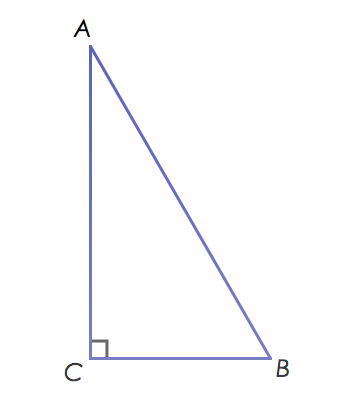
\includegraphics[scale=0.15]{example_triangle_1.png} 
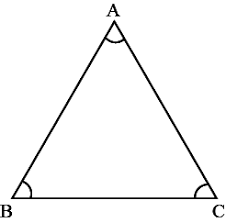
\includegraphics[scale=0.25]{example_triangle_2.png} 
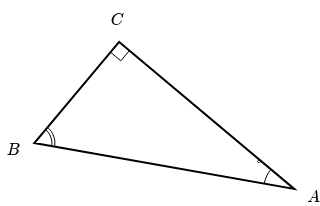
\includegraphics[scale=0.3]{example_triangle_3.png} 

\begin{figure}[ht]
  \begin{center}
  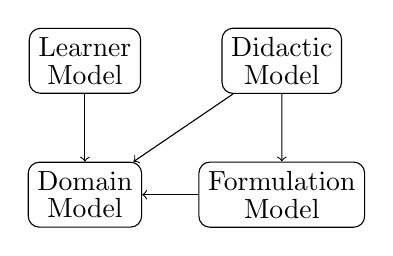
\begin{tikzpicture}[xscale=2.5,yscale=1.7]
    \node[draw,rounded corners] (dm) at (0,0) {\shortstack{Domain\\Model}};
    \node[draw,rounded corners] (lm) at (0,1) {\shortstack{Learner\\Model}};
    \node[draw,rounded corners] (fm) at (1,0) {\shortstack{Formulation\\Model}};
    \node[draw,rounded corners] (im) at (1,1) {\shortstack{Didactic\\Model}};
    \draw[->] (lm) -- (dm);
    \draw[->] (fm) -- (dm);
    \draw[->] (im) -- (dm);
    \draw[->] (im) -- (fm);
  \end{tikzpicture}
  \end{center}
  \caption{Test}
\end{figure}
\newpage

\newtcolorbox{exampleborderbox}{
  empty,
  title={Example Box},
  attach boxed title to top left,
     minipage boxed title,
  boxed title style={empty,size=minimal,toprule=0pt,top=1pt,left=3mm,overlay={}},
  coltitle=blue,fonttitle=\bfseries,
  parbox=false,boxsep=0pt,left=3mm,right=0mm,top=2pt,breakable,pad at break=0mm,
     before upper=\csname @totalleftmargin\endcsname0pt, 
  overlay unbroken={\draw[blue,line width=2pt] ([xshift=-0pt]title.north west) -- ([xshift=-0pt]frame.south west); },
  overlay first={\draw[blue,line width=2pt] ([xshift=-0pt]title.north west) -- ([xshift=-0pt]frame.south west); },
  overlay middle={\draw[blue,line width=2pt] ([xshift=-0pt]frame.north west) -- ([xshift=-0pt]frame.south west); },
  overlay last={\draw[blue,line width=2pt] ([xshift=-0pt]frame.north west) -- ([xshift=-0pt]frame.south west); },
  outer arc=4pt%
}

\definecolor{backcolor}{gray}{.96}

\begin{exampleborderbox}
  %\rustexBREAK
  \lorem
  \begin{lstlisting}[backgroundcolor=\color{backcolor},numbers=left,gobble=4,numbersep=3pt,xleftmargin=5pt,lineskip=-.7ex,alsoletter=\\]
    \newtcolorbox{exampleborderbox}{
      empty,
      title={Example Box},
      attach boxed title to top left,
        minipage boxed title,
      boxed title style={empty,size=minimal,toprule=0pt,top=1pt,
        left=3mm,overlay={}},
      coltitle=blue,fonttitle=\bfseries,
      parbox=false,boxsep=0pt,left=3mm,right=0mm,top=2pt,breakable,
        pad at break=0mm, before upper=\csname @totalleftmargin\endcsname0pt, 
      overlay unbroken={\draw[blue,line width=2pt] 
        ([xshift=-0pt]title.north west) -- ([xshift=-0pt]frame.south west); },
      overlay first={\draw[blue,line width=2pt] 
        ([xshift=-0pt]title.north west) -- ([xshift=-0pt]frame.south west); },
      overlay middle={\draw[blue,line width=2pt] 
        ([xshift=-0pt]frame.north west) -- ([xshift=-0pt]frame.south west); },
      overlay last={\draw[blue,line width=2pt] 
        ([xshift=-0pt]frame.north west) -- ([xshift=-0pt]frame.south west); },
      outer arc=4pt%
    }
  \end{lstlisting}
  \begin{mdframed}
    \lorem \lorem
  \end{mdframed}
\end{exampleborderbox}

\definecolor{bubblegreen}{RGB}{103,184,104}
\definecolor{bubblegray}{RGB}{241,240,240}

\newcommand{\bubble}[4]{%
  \tcbox[
    on line,
    arc=2mm,
    colback=#1,
    colframe=#1,
    #2,top=0pt,left=1pt,right=1pt,bottom=0pt
  ]{\color{#3}\begin{varwidth}{0.5\textwidth}#4\end{varwidth}}%
}

\noindent \bubble{bubblegreen}{rounded corners}{white}{%
  foo 
}\par

\bubble{bubblegreen}{rounded corners}{white}{\lorem}


\section{Other Stuff}

\block{\cs{raise}}{
\showpar{Bla bla \raise10pt\hbox{bla bla} bla bla
\raise-10pt\hbox{bla bla} bla bla}
}

\block{\cs{raise}}{
\showpar{\raise10pt\hbox{\lorem}}
}
\pagebreak

\block{\cs{raise}}{
\showpar{\raise-10pt\hbox{\lorem}}
}

\block{spaces}{
other test { }{ }{ }{ }{ } foo
}

\block{\cs{TeX} and \cs{LaTeX}}{
bla bla \TeX{} bla bla

bla bla \LaTeX{} bla bla
}

\block{footnotes, items}{
\begin{itemize}
  \item \lorem\footnote{Footnote 1 \lorem}
  \item \lorem
  \item \lorem \begin{itemize}
  \item \lorem
  \item \lorem\footnote{Footnote 2 \lorem}
  \item \lorem
  \end{itemize}
\end{itemize}
}

\block{empty boxes}{
\hbox to 0pt {\hbox to 200pt{%
  \setbox0\hbox{\vbox{\lorem}}
  \wd0=0pt%
  \vbox{\box0}
}}
}

\iffalse

\subsection{Peskiness}

{\Huge
  \TeX{ }\LaTeX Bla\vbox{\small\hbox{foo}}Bla%
  \vtop{\small\hbox{foo}}Bla\vbox{\small\hbox{foo}\vss}Bla%
  \vtop{\small\hbox{foo}\vss}
}




\iffalse
\begin{flushright}
  \begin{varwidth}{0.5\textwidth} \lorem\lorem\lorem \end{varwidth}
\end{flushright}

\setbox0\vbox{foo}\the\wd0

\setbox0\hbox{$\vcenter{foo}$}\the\wd0

\noindent foo \setbox0\vbox{foo}\the\wd0

\noindent foo \setbox0\hbox{$\vcenter{foo}$}\the\wd0

\par




\vbox{
  \noindent \lorem\lorem\lorem \par
  \setbox0\lastbox
  \hbox{\the\wd0, \ifvbox0V\else H\fi}
  \setbox0\hbox{\unhbox0}
  \hbox{\the\wd0, \ifvbox0V\else H\fi}

  \rustexBREAK
  \noindent Foo \par
  \begingroup
  \setbox0\lastbox
  \hbox{\the\wd0, \ifvbox0V\else H\fi}
  \setbox0\hbox{\unhbox0}
  \hbox{\the\wd0, \ifvbox0V\else H\fi}
  \endgroup
}
\fi

\iffalse

\makeatletter
\newcommand{\oset}[3][0ex]{
	\mathrel{\mathop{#3}\limits^{\vbox to#1{\kern-2\ex@\hbox{$\scriptstyle#2$}}}}
}
\makeatother

$\oset[-.45ex]\Rightarrow\equiv$

\fi

\iffalse
$ a \begin{array}{l} \alpha+\beta \\ \alpha \end{array} b $
$ a \begin{array}{c} \alpha+\beta \\ \alpha \end{array} b $
$ a \begin{array}{r} \alpha+\beta \\ \alpha \end{array} b $

\begin{itemize}
  \item We prove $\neg(\forall X.P(X))\vdash_{\mathcal{ND}^1}\exists X.\neg P(X)$.
  \begin{displaynd}
    \ian{\ian{\ibn{\neg\forall X. P(X)}
                          {\ian{\ian{\ian{\ibn{[\neg\exists X. \neg P(X)]^1}
                                                {\ian{[\neg P(X)]^2}
                                                        {\exists X \neg P(X)}
                                                        {\exists I}}
                                                {F}
                                                {FI}}
                                         {\neg\neg P(X)}
                                         {\neg I^2}}
                                 {P(X)}
                                 {\neg E}}
                                 {\forall X. P(X)}
                          {\forall I}} 
                          {F}
                          {FI}}
                   {\neg\neg\exists X.\neg P(X)}
                   {\neg I^1}}
           {\exists X. \neg P(X)}
           {\neg E}
  \end{displaynd}
\end{itemize}

\begin{center}\small
  \begin{tabular}{c|c}
  \textbf{Abstract Syntax} & \textbf{Scala Syntax} \\\hline\hline
  Symbol References $S$ & \lstinline*OMID(S : ContentPath)*  \\
  Module References $M$ & \rustexBREAK \lstinline*OMMOD(M : MPath)*\rustexBREAK = \lstinline*OMID(M)*\rustexBREAK  \\
  Constant References $C$ & \lstinline*OMS(C : GlobalName)* = \lstinline*OMID(C)*  \\
  Variable References $V$ & \lstinline*OMV(V : LocalName)*  \\\hline
  Applications $f({a_1,\ldots,a_n})$ & \lstinline*OMA(f : Term, args : List[Term])* \\
  Binding Applications $f{{con}}{{arg}}$ & \lstinline*OMBIND(f : Term, con : Context, arg: Term)* \\\hline
  Context $G=\{{vars}\}$ & \lstinline*Context(vars : List[VarDecl])* \\
  Variable Declaration $v[:t][:=d]$ & \lstinline*VarDecl(v : LocalName, t : Option[Term], d : Option[Term])* \\ 
  \end{tabular}
\end{center}

\noindent left: \the\leftskip; right: \the\rightskip

\begin{center}
  \noindent left: \the\leftskip; right: \the\rightskip

  \begin{tabular}{l|l}
    left & right \\
    \the\leftskip & \the\rightskip 
  \end{tabular}
  
  \begin{tabular}{c|c}
    left & right \\
    \the\leftskip & \the\rightskip 
  \end{tabular}

  \begin{tabular}{c|c}
    left & right \\
    \vbox{\noindent \the\leftskip} & \the\rightskip 
  \end{tabular}

  \begin{tabular}{c|c}
    left & right \\
    \hbox{\vbox{\noindent \the\leftskip}\hss} & \the\rightskip 
  \end{tabular}

  \begin{tabular}{c|c}
    left & right \\
    \hbox to 0pt{\vbox{\noindent \the\leftskip}} & \the\rightskip 
  \end{tabular}

\end{center}

\fi

\iffalse

\hbox{\hbox{testa}\lower10pt\hbox{testb}\hbox{testc}}
\hbox{\hbox{testa}\hbox{testb}\hbox{testc}}
\hbox{\hbox{testa}\hbox{testb}\hbox{testc}}
\hbox{\hbox{testa}\raise10pt\hbox{testb}\hbox{testc}}
%\hbox{\hbox{testa}\moveleft10pt\hbox{testb}\hbox{testc}}
%\hbox{\hbox{testa}\moveright10pt\hbox{testb}\hbox{testc}}
\hbox{
\vbox{\hbox{testa}\hbox{testb}\hbox{testc}}
\vbox{\moveleft20pt\hbox{testa}\hbox{testb}\moveright30pt\hbox{testc}}
\vbox{\hbox{testa}\hbox{testb}\hbox{testc}}
}
\hbox{
\vbox{\hbox{testa}\hbox{testb}\hbox{testc}}
\vbox{\moveright-20pt\hbox{testa}\hbox{testb}\moveleft-30pt\hbox{testc}}
\vbox{\hbox{testa}\hbox{testb}\hbox{testc}}
}
\fi

\fi


\vfill

\end{document}
